%Matteo Kumar - Leonard Schatt
% Fortgeschrittenes Physikalisches Praktikum

% Teilauswertung Nanoröhrchen

\section{Nanoröhrchen}
Dieser Versuchsteil widmet sich der Untersuchung der Nanoröhrchen. Diese sind Kohlenstoffnanoröhre, welche auf einem Silizium-Waver 
fixiert wurden. Ziel diese Versuchsteiles ist es den Krümmungsradius der Spitze zu bestimmen.
\subsection{Länge und Durchmesser}
\subsubsection*{Länge}
Um die Länge einzelner Nanoröhrchen zu bestimmen, haben wir eine Aufnahme mit 15 $\mu$m als Seitenlängen gemacht. In dieser haben wir uns 
dann angeschaut, welche Längen unterschiedlich lange Kohlenstoffnanoröhren haben. Dazu bestimmt man mit dem Distanzmessen-Tool der Software 
"Gwyddion" die Länge möglichst gerader Nanoröhrchen bestimmt. \\
Die Abbildung \ref{Nanotube20} zeigt die oben genannte Aufnahme. Dabei kann man sehr schön die langgezogenen Fäden sehen. Welche dabei zum Vermessen verwendet wurden, 
kann man Abbildung \ref{Nanotube20Mess} im Anhang entnehmen.

\begin{figure}[h]
    \centering
    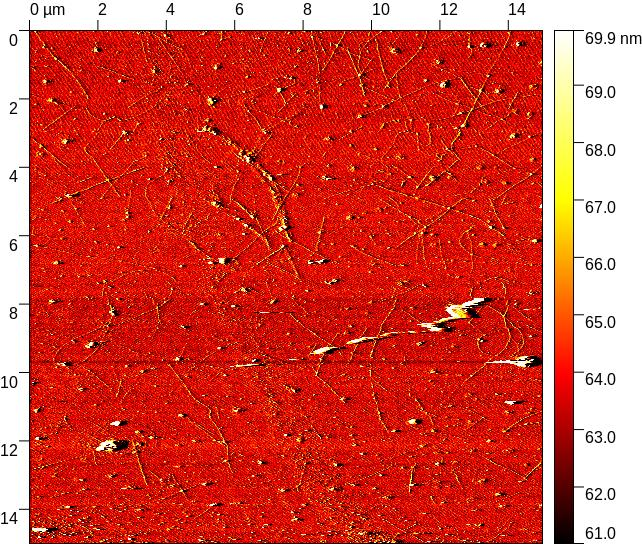
\includegraphics[width = 9cm]{Bilder/Nanotubes/NanoTube15um.jpg}
    \caption{Nanoröhrchen bei einer Bildgröße von 15x15$\mu$m}
    \label{Nanotube20}
\end{figure}

Dabei wurden folgende Werte aus Tabelle \ref{TabLaenge} gemessen. Die Fehlerrechnung kann man bei diesem 
Versuchsteil vernachlässigen, weil die Ablesefehler so groß sind, dass der Fehler des Messgeräts vernachlässigbar klein ist. Der Ablesefehler wird auf 15\% der Länge geschätzt. \\

\begin{table}
    \centering
    \begin{tabular}{lr}
        \toprule
        Röhrennummer &   Länge ($\mu$ m) \\
        \midrule
        0  &  2.883 $\pm$ 0.43 \\
        1  &  2.374 $\pm$ 0.35\\
        2  &  1.334 $\pm$ 0.20 \\
        3  &  3.050 $\pm$ 0.46 \\
        4  &  3.753 $\pm$ 0.56 \\
        5  &   0.860 $\pm$ 0.12\\
        6  &  1.583 $\pm$ 0.24 \\
        7  &  1.896 $\pm$ 0.28 \\
        8  &  1.542 $\pm$ 0.23 \\
        9  &   0.590 $\pm$ 0.075 \\
        10 &   0.464 $\pm$ 0.070 \\
        11 &  4.412 $\pm$ 0.66\\
        \bottomrule
    \end{tabular}
    \caption{Längenmessung der Nanoröhrchen. Der Ablesefehler wird auf 15\% der Länge geschätzt. \\
    }
    \label{TabLaenge}
\end{table}

Man erkennt, dass die Röhren sehr stark in ihrer Länge $l$  variieren.

\begin{equation}
    \textcolor{red}{\frac{l_{Min}}{l_{Max}} = 0.1053209772450975}
\end{equation}

Die maximale relative Unterschied in der Länge $l$ liegt bei einem Faktor 10. Dabei sind die Längen für die langen 
Nanoröhrchen, welche wir gemessen haben, noch nicht mal besonders lang. Diese können in Extremfällen bis zu
einen halben Meter lang werden (\cite{Dagani2002}).

\subsection*{Radius der Röhre}

Man muss sich Nanoröhrchen wie lange Röhren vorstellen, welche eine kreisförmige Grundfläche haben. Von dieser wollen wir nun den 
Radius bestimmen. Da das Abtasten aber einen Kreis mit anderem Radius ergibt muss man statt diesen Radius zu bestimmen, einfach 
den Höhenunterschied der des Hochpunktes der Röhre zum normalen untergrund bestimmen. Leider ist der Untergrund des Silizium-Wavers 
keineswegs glatt; deshalb ist es schwer den Unterschied exakt zu messen. Der Fehler im Ablesen der Werte dominiert den Fehler bei weitem. 
\begin{figure}
    \centering
    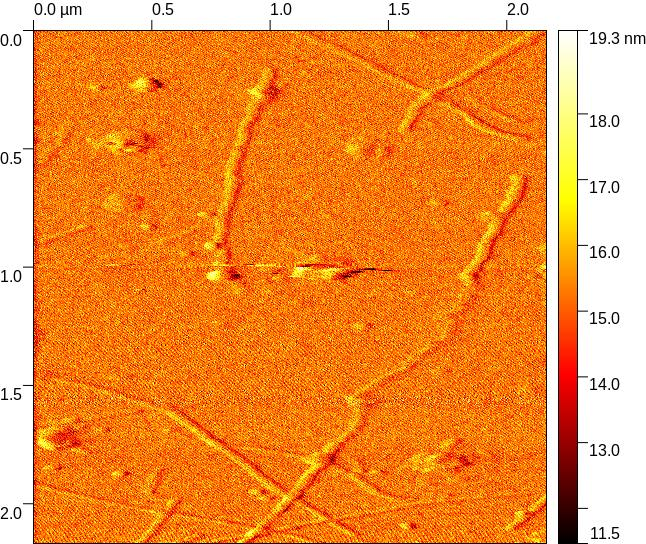
\includegraphics[width = 9cm]{Bilder/Nanotubes/NanoTube2um.jpg}
    \caption{Nanoröhrchen in einer Auflösung mit 512x512 Bildpunkten auf 2x2$\mu$m}
\end{figure}

Zur Bestimmung des Radius wird ein Röhrchen senkrecht mit einer Linie geschnitten. Auf dieser Linie betrachtet man dann das Höhenprofil der Aufnahme. Wir haben dafür die 
Linie, wie in Abbildung \ref{NanoRadius} zu sehen, gewählt. Damit erhält man den Querschnitt, der in Abbildung \ref{NanoQuerschnitt} 
dargestellt wird.

\begin{figure}
    \centering
    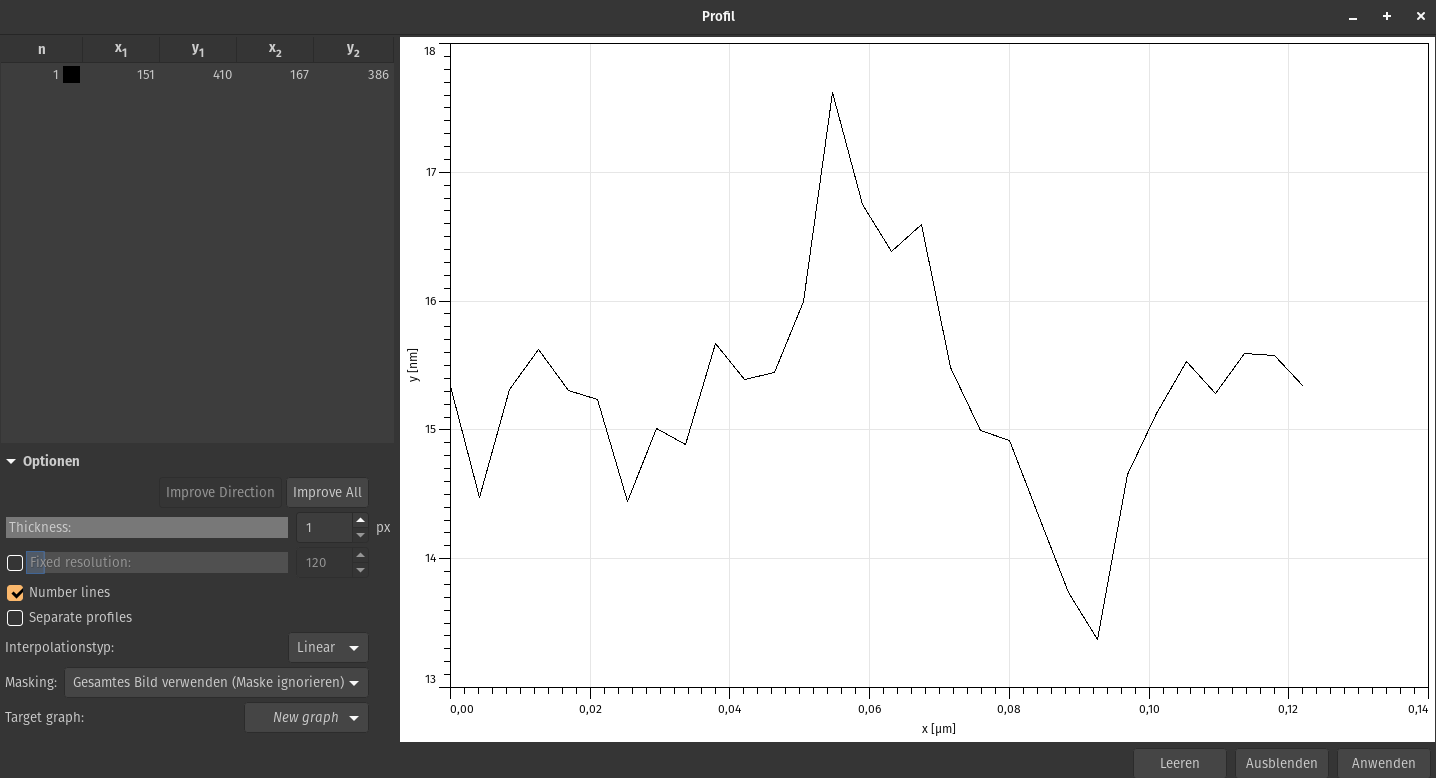
\includegraphics[width = \linewidth]{Bilder/Nanotubes/NanotubesBreiteHoehe.png}
    \caption{Querschnitt eins Kohlenstoffröhrchens}
    \label{NanoQuerschnitt}
\end{figure}

Aus diesem bestimmt man grafisch den Höhenunterschied. Dieser entspricht dann zwei Mal dem Radius $r$ der Röhre. Dabei wird der Fehler 
großzügig mit 15\% des Wertes angegeben.

\begin{equation*}
   r = \frac{\Delta z}{2} = \frac{2,6\mathrm{nm}}{2} = 1,3\mathrm{nm}
\end{equation*}

Durch das halbieren halbiert sich auch der Ablesefehler. 
\begin{equation*}
    \Rightarrow \textcolor{red}{r = (1,300 \pm 0,098)\mathrm{nm}}
\end{equation*}


\subsection{Krümmungsradius der Spitze des Cantilevers}

Wie oben beschrieben sagt die Form der Abtastung etwas über den Krümmungsradius der Spitze des Cantilevers aus. Das wird in Abbildung 
\ref{NanoTip} anschaulich dargestellt.

\begin{figure}
    \centering
    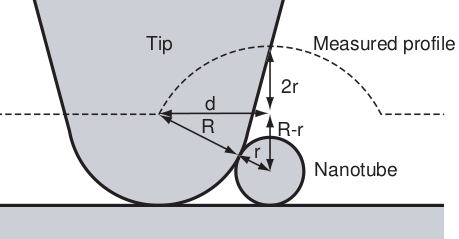
\includegraphics[width = 10cm]{Bilder/Nanotubes/TipGeoNano.png}
    \caption{Zusammenhang Krümmungsradius $R$ der Spitze und Präparatradius $r$ aus der abgebildeten Kontur (\cite[S.46]{SampleKit2007})}
    \label{NanoTip}
\end{figure}

Darau ergibt sich für den Radius der Spitze (\cite[S.47]{SampleKit2007}):\\
\begin{equation}
    R = \frac{d^2}{4r}
\end{equation}
mit $d$, $R$ und $r$ wie in Abbildung\ref{NanoTip} eingezeichnet.

Auch für $d$ setzt man beim Ablesen am besten ein großzügiges Intervall der Unsicherheit von 50\% an, da es schwer ist aus 
dem Rauschen herauszulesen, wo der Peak anfängt. Abgelesen wurde:\\

\begin{equation*}
    2d = 25,0\pm12,5\mathrm{nm} \Rightarrow d = (12,5\pm 6,3) \mathrm{nm} 
\end{equation*}

Daraus ergibt sich mit dem Fehlerfortpflanzungsgesetz:\\

\begin{equation}
    \textcolor{red}{R = (30\pm15) \mathrm{\,nm}}
\end{equation}

Das scheint ein in der Größenordnung realistischer Wert. Die Spitze könnte noch gut sein. Für eine Spitze sind Krümmungsradien zwischen 
10 und 20 nm normal. Die Spitze tendiert aber dazu, etwas abgenutzt zu sein.